\chapter{Tat}
\section{Analysis of Fixed Angle Data using NFIT}\label{sec:fixed_angle_analysis}
In this section, I propose a slightly new method to analyze the diffuse 
scattering data. This method may allow us to measure the X-ray form factor
at lower $q_z$ than we have traditionally measured. 

\subsection{Theory}

\subsection{Results}

\section{Proper Incorporation of Mosaic Spread to NFIT analysis}
\label{sec:mosaic_spread}
First we describe the theory of mosaic spread for diffuse scattering. 
Next we discuss some simplification. Third, we discuss the program.
Fourth, we show the results.

\subsection{Mosaic Spread: Calculation}
(Some things are messed up.)
In this section, an analytical framework for a measurement of mosaic spread will 
be developed. Let us imagine that a sample is made up of many small domains 
that are 
tilted from the direction perpendicular to the substrate normal by some amount. 
A "perfect" domain is a domain that is parallel to the substrate plane.
Then, we can consider a probability distribution function, $P(\alpha)$, 
representing a probablity of finding a domain with tilt $\alpha$, which is the 
angle
between the substrate normal and the tilted domain normal. Here, we have
assumed the rotational symmetry about the substrate normal, so that the 
distribution
does not depend on the azimuthal angle, $\beta$. The normalization condition on 
the probability distribution is 
\begin{equation}
  1 = \int_0^{2\pi} \!\! \mathrm{d}\beta  
      \int_0^{\frac{\pi}{2}} \! \mathrm{d}\alpha \, \sin\alpha \, P(\alpha).
\end{equation}
The object of this section is to derive the x-ray scattering structure factor 
including the probability distribtion. The cooridate system employed here is 
such that x, y, and
z-axes of the zero tilt domain, that is, a domain parallel to the substrate, 
coincide with the lab x, y, and z-axes 

First, we want to calculate the structure factor for a domain tilted by 
$\alpha$ and $\beta$, expressed in the lab coordinates (Need a figure). 
For this, we need to express
$\mathbf{q}$ in terms of . We imagine
rotating the coorinates about the y-axis first, and then about the z-axis. In
other words, we apply the appropriate rotation matrices to , y, and 
z-axes. The rotation matrix for rotaing a vector about y-axis is given by
\begin{equation}
  \begin{pmatrix} 
    \cos\alpha & 0 & -\sin\alpha \\ 
    0 & 1 & 0 \\
    \sin\alpha & 0 & \cos\alpha 
  \end{pmatrix}
\end{equation}
and for ratating about z-axis
\begin{equation}
  \begin{pmatrix} 
    \cos\beta & \sin\beta & 0 \\ 
    -\sin\beta & \cos\beta & 0 \\
    0 & 0 & 1 
  \end{pmatrix}
\end{equation}
Then, what we want is
\begin{equation}
  \mathbf{\hat{x}}' = 
  \begin{pmatrix} 
    \cos\beta & \sin\beta & 0 \\ 
    -\sin\beta & \cos\beta & 0 \\
    0 & 0 & 1 
  \end{pmatrix}
  \begin{pmatrix} 
    \cos\alpha & 0 & -\sin\alpha \\ 
    0 & 1 & 0 \\
    \sin\alpha & 0 & \cos\alpha 
  \end{pmatrix}
  \begin{pmatrix}
    1 \\
    0 \\
    0
  \end{pmatrix}
  = 
  \begin{pmatrix}
    \cos\alpha\cos\beta \\
    \cos\alpha\sin\beta \\
    -\sin\alpha
  \end{pmatrix}
\end{equation}
\begin{equation}
  \mathbf{\hat{y}}' = 
  \begin{pmatrix} 
    \cos\beta & \sin\beta & 0 \\ 
    -\sin\beta & \cos\beta & 0 \\
    0 & 0 & 1 
  \end{pmatrix}
  \begin{pmatrix} 
    \cos\alpha & 0 & -\sin\alpha \\ 
    0 & 1 & 0 \\
    \sin\alpha & 0 & \cos\alpha 
  \end{pmatrix}
  \begin{pmatrix}
    0 \\
    1 \\
    0
  \end{pmatrix}
  =
  \begin{pmatrix}
    -\sin\beta \\
    \cos\beta \\
    0
  \end{pmatrix}
\end{equation}
\begin{equation}
  \mathbf{\hat{z}}' = 
  \begin{pmatrix} 
    \cos\beta & \sin\beta & 0 \\ 
    -\sin\beta & \cos\beta & 0 \\
    0 & 0 & 1 
  \end{pmatrix}
  \begin{pmatrix} 
    \cos\alpha & 0 & -\sin\alpha \\ 
    0 & 1 & 0 \\
    \sin\alpha & 0 & \cos\alpha 
  \end{pmatrix}
  \begin{pmatrix}
    0 \\
    0 \\
    1
  \end{pmatrix}
  =
  \begin{pmatrix}
    \sin\alpha\cos\beta \\
    \sin\alpha\sin\beta \\
    \cos\alpha
  \end{pmatrix}
\end{equation}
Then, the components of $\mathbf{q}$ represented in the rotated coodinates, 
denoted 
by $\mathbf{q'}$, are the projection of $\mathbf{q}$ on x$'$, y$'$, and 
z$'$-axes, 
that is,
\begin{equation}
  q_x' = \mathbf{q} \cdot \mathbf{\hat{x}'} 
       = q_x\cos\alpha\cos\beta + q_y\cos\alpha\sin\beta -q_z\sin\alpha  
\end{equation}
\begin{equation}
  q_y' = \mathbf{q} \cdot \mathbf{\hat{y}'} 
       = -q_x\sin\beta + q_y\cos\beta  
\end{equation}
\begin{equation}
  q_z' = \mathbf{q} \cdot \mathbf{\hat{z}'} 
       = q_x\sin\alpha\cos\beta + q_y\sin\alpha\sin\beta + q_z\cos\alpha  
\end{equation}
The transformation rule we are looking for is 
\begin{equation}
  \cos\theta' = \frac{q_z'}{q} 
              = \sin\theta\sin\alpha\cos(\phi-\beta) + \cos\theta\cos\alpha 
  \label{eq:theta'}
\end{equation}
and
\begin{equation}
  \tan\phi' 
    = \frac{q_y'}{q_x'}
    = \frac{\sin\theta\sin(\phi-\beta)}{\sin\theta\cos\alpha\cos(\phi-\beta) 
                                       -\cos\theta\sin\alpha}
  \label{eq:phi'}
\end{equation}
The structure factor of the tilted domain in the lab coordinates is simply 
given 
by $S(\mathbf{q'})=S(q,\theta',\phi')$. Summing over all the domains, we get 
for the total structure factor
\begin{equation}
  S_M(q,\theta,\phi) = \int_0^{2\pi}\mathop{d\beta} \int_0^{\frac{\pi}{2}} 
  \mathop{d\alpha} S(q,\theta',\phi')P(\alpha)
  \label{eq:SM}
\end{equation}
with Eq.\,(\ref{eq:theta'}) and Eq.\,(\ref{eq:phi'}).

Given Eqs.\,(\ref{eq:theta'}), (\ref{eq:phi'}), and (\ref{eq:SM}), we want to
 show that
mosaic spread acts as one dimensional convolution in the x-ray structure factor:
\begin{equation}
  S_M(q,\theta) 
    = \int_{-\pi}^{\pi} \mathrm{d}\alpha \, S(q,\theta-\alpha) \, P(\alpha)
  \label{eq:conv}
\end{equation}
The structure factor representing Bragg peaks in the spherical coordinates are 
written as
\begin{equation}
  S(q,\theta,\phi) 
    \sim \frac{\delta(q-\frac{2\pi h}{D})}{q^2} 
         \delta(\cos\theta-1) \delta(\phi)
  \label{eq:Bragg}
\end{equation}
where $\delta(x)$ is the Dirac delta function. Plugging \Eq{eq:Bragg} in 
\Eq{eq:SM},
we obtain $\phi-\beta=0$. Using this condition, we get 
\begin{equation}
  S_M(q,\theta) \sim \frac{\delta(q-\frac{2\pi h}{D})}{q^2}P(\theta),
\end{equation}
which shows that we can directly measure the probability distribution 
experimentally
by looking at the intensity along $q=2\pi h/D$. In the next section, we will 
discuss 
the relevant experimental techniques.

\subsection{Mosaic Spread: Experiment}
(Under construction)
In this section, we discuss experimental procedures to probe appropriate 
$q$-space
to measure the mosaic distribution, $P(\alpha)$. In our setup, the angle of 
incidence between the beam and substrate, denoted by $\omega$, can be varied. A 
conventional method to measure mosaicity distribution is a rocking scan, where
one measures the integrated intensity of a given Bragg peak as a function of 
$\omega$ with a fixed detector position. In a non-conventional method called
ring analysis, one measures the intensity as a function of $\eta$ on a two
dimensional detector. First, we want to compare the two methods mentioned 
above and figure out the exact relationship between them.

\begin{figure}
  \centering
  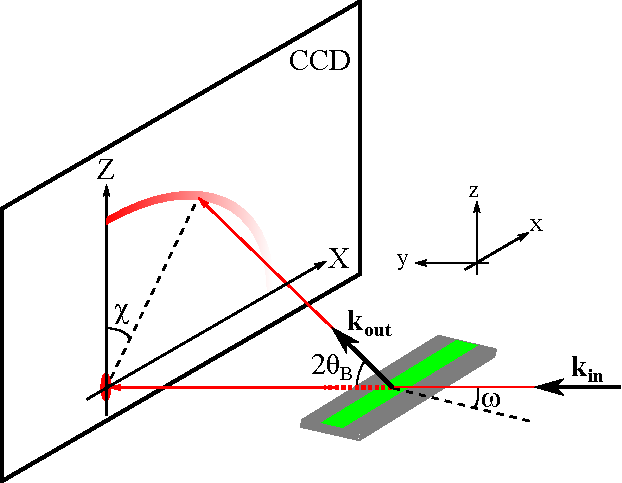
\includegraphics[width=0.8\textwidth]{figures/ripple/mosaic/ring_setup}
  \caption{Notations used in this section. The arc originating from the $Z$-axis
  is the mosaic arc due to the mosaic spread distribution.}
  \label{fig:ring_setup}
\end{figure}


Using the coordinates defined in Fig.~\ref{fig:ring_setup},
borrowing Eq.~(\ref{eq:qxqyqz}), and replacing $\phi=\pi/2-\chi$,
we have
\begin{align}
  q_x &= q\cos\theta\sin\chi, \nonumber\\
  q_y &= q\left(-\sin\theta\cos\omega + \cos\theta\cos\chi\sin\omega\right), \nonumber\\
  q_z &= q\left(\sin\theta\sin\omega + \cos\theta\cos\chi\cos\omega\right),
  \label{eq:ccd2q}
\end{align}
or in the small angle approximation,
\begin{align}
  q_x &\approx \frac{4\pi\theta\sin\chi}{\lambda} \approx kX/S \nonumber\\
  q_y &\approx q_z\omega -\frac{4\pi\theta^2}{\lambda} \approx q_z\omega - \frac{\lambda q_z^2}{4\pi}\nonumber\\
  q_z &\approx \frac{4\pi\theta\cos\chi}{\lambda} \approx kZ/S.
  \label{eq:ccd2q_small}
\end{align}
For a rocking scan focused on a particular order, 
$\chi=0$ and $\theta=\theta_B$ while $\omega$ is varied about $\theta_B$, 
where $\theta_B$ is the Bragg angle. Then, 
\begin{align}
  q_x &= 0 \nonumber\\
  q_y &= q\sin(\omega-\theta_B) \nonumber\\
  q_z &= q\cos(\omega-\theta_B),
  \label{eq:rock} 
\end{align}
which shows that this scan traces a circular path in the $q_x=0$ plane.


\subsection{Results}

\section{Domain Size Distribution: Gaussian and Exponential}

\section{Hard Wall Constraints in SDP}

\section{Some More Details of Tat Stuff}

\chapter{Ripple Phase}
\section{Derivation of the contour part of the form factor}
In this section, we derive $\FC$. The ripple profile, $u(x)$ is given by
\begin{equation}
  u(x) = \left\{
    \begin{array}{ccc}
    -\frac{A}{\lambda_r-x_0}\left(x+\frac{\lambda_r}{2}\right) 
      & \text{for} 
      & -\frac{\lambda_r}{2} \leq x < -\frac{x_0}{2} \\
    \frac{A}{x_0}x 
      & \text{for} 
      & -\frac{x_0}{2} \leq x \leq \frac{x_0}{2} \\
    -\frac{A}{\lambda_r-x_0} \left(x-\frac{\lambda_r}{2}\right)
      & \text{for} 
      & \frac{x_0}{2} < x \leq \frac{\lambda_r}{2}
    \end{array} \right.
\end{equation}

The contour part of the form factor is the Fourier transform of the contour
function, $C(x,z)$,
\[
  \FC(\mathbf{q}) = \frac{1}{\lambda_r}
  \int_{-\frac{\lambda_r}{2}}^{\frac{\lambda_r}{2}}\dx
  \int_{-\frac{D}{2}}^\frac{D}{2}\dz 
  C(x,z) e^{iq_zz} e^{iq_xx}
\] 
As discussed in section X, the modulated models allow
the electron density to modulate along the ripple direction, $x$. This means
\begin{align}
  C(x,z) &= \left\{
  \begin{array}{ccc}
    f_1\delta[z-u(x)] & \text{for} & -\frac{\lambda_r}{2} \leq x < -\frac{x_0}{2} \\
    \delta[z-u(x)] & \text{for} & -\frac{x_0}{2} < x < \frac{x_0}{2} \\
    f_1\delta[z-u(x)] & \text{for} & \frac{x_0}{2} \leq x < \frac{\lambda_r}{2} \\    
  \end{array}
  \right. \nonumber\\
  &+ f_2\,\delta\!\pars{x+\frac{x_0}{2}}\delta\!\pars{z+\frac{A}{2}} 
   + f_2\,\delta\!\pars{x-\frac{x_0}{2}}\delta\!\pars{z-\frac{A}{2}}.
\end{align}
The contribution from the minor arm is
\begin{align}
  & \frac{1}{\lambda_r}
  \int_{-\frac{\lambda_r}{2}}^{-\frac{x_0}{2}}\dx e^{iq_xx} e^{iq_zu(x)}
  + \int_{\frac{x_0}{2}}^{\frac{\lambda_r}{2}}\dx e^{iq_xx} e^{iq_zu(x)} \nonumber\\
  &= \frac{1}{\lambda_r}
     \int_{\frac{x_0}{2}}^{\frac{\lambda_r}{2}}\dx 
     e^{-i\left[q_xx-q_z\frac{A}{\lambda_r-x_0}\left(x-\frac{\lambda_r}{2}\right)\right]}
     + \int_{\frac{x_0}{2}}^{\frac{\lambda_r}{2}}\dx 
     e^{i\left[q_xx-q_z\frac{A}{\lambda_r-x_0}\left(x-\frac{\lambda_r}{2}\right)\right]} \nonumber\\
  &= \frac{2}{\lambda_r}
     \int_{\frac{x_0}{2}}^{\frac{\lambda_r}{2}}   
     \cos\bracks{\pars{q_x-q_z\frac{A}{\lambda_r-x_0}}x
                 +q_z\frac{A}{\lambda_r-x_0}\frac{\lambda_r}{2}} \label{eq:minor_arm1}
\end{align}
Using a trigonometric identity, 
\[
  \sin u-\sin v = 2\cos[(u+v)/2]\sin[(u-v)/2],
\]
and defining 
\begin{equation}
  \omega(\mathbf{q}) = \frac{1}{2}\left(q_xx_0 + q_zA\right),
\end{equation}
we further simplify Eq.~(\ref{eq:minor_arm1}),
\begin{align}
  &= \frac{2}{\lambda_r}\frac{\lambda_r-x_0}{\frac{1}{2}q_x\lambda_r - \omega} 
     \cos\bracks{\frac{1}{2}\left(\frac{1}{2}q_x\lambda_r + \omega\right)} 
     \sin\bracks{\frac{1}{2}\left(\frac{1}{2}q_x\lambda_r - \omega\right)} \nonumber\\
  &= \frac{1}{\lambda_r}\frac{\lambda_r-x_0}{\frac{1}{2}q_x\lambda_r - \omega} 
     \cos\bracks{\frac{1}{2}\left(\frac{1}{2}q_x\lambda_r + \omega\right)} 
     \frac{\sin\left(\frac{1}{2}q_x\lambda_r - \omega \right)}
          {\cos\bracks{\frac{1}{2}\left(\frac{1}{2}q_x\lambda_r - \omega\right)}} \nonumber\\
  &= \frac{\lambda_r-x_0}{\lambda_r}
     \frac{\cos\bracks{\frac{1}{2}\left(\frac{1}{2}q_x\lambda_r + \omega\right)}}
          {\cos\bracks{\frac{1}{2}\left(\frac{1}{2}q_x\lambda_r - \omega\right)}}
     \frac{\sin\left(\frac{1}{2}q_x\lambda_r - \omega\right)}
          {\frac{1}{2}q_x\lambda_r - \omega}.
\end{align}
Similarly, we calculate the contribution from the major arm,
\begin{align}
  \frac{1}{\lambda_r}\int_{-\frac{x_0}{2}}^{\frac{x_0}{2}}\dx 
  e^{i\left(\frac{q_zA}{x_0} + q_x \right)x}
  &= \frac{2}{\lambda_r}\int_{0}^{\frac{x_0}{2}}\dx \cos\left(\frac{q_zA}{x_0} + q_x\right)x \nonumber\\ 
  &= \frac{x_0}{\lambda_r}\frac{\sin\omega}{\omega}
\end{align}
The contribution from the kink region is 
\begin{align}
  & \frac{1}{\lambda_r}\iint\dx\dz
  \bracks{\delta\!\pars{x+\frac{x_0}{2}}\delta\!\pars{z+\frac{A}{2}} 
   + \delta\!\pars{x-\frac{x_0}{2}}\delta\!\pars{z-\frac{A}{2}}}
  e^{iq_xx} e^{iq_zz} \nonumber\\
  &= \frac{2}{\lambda_r}\cos\omega.
\end{align}
Therefore,
\begin{align}
  \FC(\mathbf{q}) 
  &= \frac{x_0}{\lambda_r}\frac{\sin\omega}{\omega} + 
  f_1\frac{\lambda_r-x_0}{\lambda_r}
  \frac{\cos\bracks{\frac{1}{2}\left(\frac{1}{2}q_x\lambda_r + \omega\right)}}
       {\cos\bracks{\frac{1}{2}\left(\frac{1}{2}q_x\lambda_r - \omega\right)}}
  \frac{\sin\left(\frac{1}{2}q_x\lambda_r - \omega\right)}
       {\frac{1}{2}q_x\lambda_r - \omega} \nonumber\\
  &+ \frac{2f_2}{\lambda_r}\cos\omega
\end{align}

%%%%%%%%%%%%%%%%%%%%%%%%%%%%%%%%%%%%%%%%%%%%%%%%%%%%%%%%%%%%%%%%%%%%%%%%%%%%%%%
\section{Rotation of a Two-Dimensional Function}
Let us consider rotating a function, $f(x,z)$ in two dimensions by an angle, 
$\psi$, in the counterclockwise direction (see Fig. X). This is easily 
achieved by rotating the coordinate system by $\psi$ in the clockwise direction. 
Let rotated coordinates be $x'$ and $z'$. A point in the original coodinates,
($x$, $z$), is written as ($x'$, $z'$) in the new coordinates. More specifically,
the point P is written as 
$\mathbf{P}=x\xhat+z\zhat=x'\xhat'+z'\zhat'$. $\xhat$ and $\zhat$ in
the $x'z'$ coordinate system are written as 
\begin{align}
  \xhat &= \cos\psi\xhat'+\sin\psi\zhat' \\
  \zhat &= -\sin\psi\xhat'+\cos\psi\zhat'.
\end{align}
Pluggin these in $\mathbf{P}=x\xhat+z\zhat$ leads to
\begin{align}
  x' &= x\cos\psi - z\sin\psi \\
  z' &= z\cos\psi + x\sin\psi,
\end{align}
the inverse of which is
\begin{align}
  x &= x'\cos\psi + z'\sin\psi \\
  z &= -x'\sin\psi + z'\cos\psi.
\end{align}
Using the latter equations, $f(x,z)$ can be expressed in terms of $x'$ and $z'$. 
The resulting function $f(x',z')$ is the rotated version of $f(x,z)$. 

As an 
example, let us consider a Dirac delta function located at $(x,z)=(0,\zh)$,
that is, $f(x,z)=\delta(x)\delta(z-\zh)$. After the rotation by $\psi$, it 
becomes
\begin{align*}
  f(x,z) 
  &\rightarrow 
    \delta(x\cos\psi+z\sin\psi) \delta(-x\sin\psi+z\cos\psi-\zh) \\
  &= \frac{\delta(x+z\tan\psi)}{|\cos\psi|}
     \frac{\delta(-x\sin\psi\cos\psi+z\cos^2\psi-\zh\cos\psi)}{1/|\cos\psi|} \\
  &= \delta(x+z\tan\psi)\delta(z\tan\psi\sin\psi\cos\psi+z\cos^2\psi-\zh\cos\psi) \\
  &= \delta(x+z\tan\psi)\delta(z-\zh\cos\psi),
\end{align*}
which is a part of the expression for $T_\psi(x,z)$ in the simple delta 
function model.

%%%%%%%%%%%%%%%%%%%%%%%%%%%%%%%%%%%%%%%%%%%%%%%%%%%%%%%%%%%%%%%%%%%%%%%%%%%%%%%
\section{Derivation of the transbilayer part of the form factor in the 2G hybrid model}
In this section, we derive the trasbilayer part of the form factor calculated
from the 2G hybrid model discussed in section X.
Defining $z'=-x\sin\psi+z\cos\psi$, the Fourier transform of a Gaussian function 
along the line tilted from $z$-axis by $\psi$ is
\begin{align}
  & \iint\dz\dx \rhoh{i} \exp\braces{-\frac{(z'-\zh{i})^2}{2\sigmah{i}^2}}
  \delta(x\cos\psi+z\sin\psi)e^{iq_xx}e^{iq_zz} \nonumber\\
  &= \frac{1}{\cos\psi}\int_{-\frac{D}{2}}^{\frac{D}{2}}\dz \rhoh{i} \exp\braces{
    -\frac{(z-\zh{i}\cos\psi)^2}{2\sigmah{i}^2\cos^2\psi} + i(q_z-q_x\tan\psi)z
  } \nonumber \\
  &\approx \rhoh{i}\sqrt{2\pi}\sigmah{i} \,\mathrm{exp}
  \braces{
    i\alpha\zh{i} - \frac{1}{2}\alpha^2\sigmah{i}^2
  } \label{eq:gauss_FT}
\end{align}
with $\alpha=q_z\cos\psi-q_x\sin\psi$.
Using Eq.~(\ref{eq:gauss_FT}) and adding the other side of the bilayer and
the terminal methyl term, we get
\begin{multline}
  F_\mathrm{G} = \sqrt{2\pi}
  \Bigg[
    -\rhom\sigmam \exp\braces{
      -\frac{1}{2}\alpha^2\sigmam^2
    } \\
    + \sum_{i=1}^{1\text{ or }2}2\rhoh{i}\sigmah{i}
    \cos(\alpha\zh{i})
    \,\mathrm{exp}\braces{-\frac{1}{2}\alpha^2\sigmah{i}^2}
  \Bigg].
\end{multline}
The strip part of the 
model in the minus fluid convention is
\begin{equation}
  \rhos(z) = \left\{
    \begin{array}{ccc}
      -\Delta\rho & \text{for } & 0 \leq z < \zchtwo\cos\psi, \\
      0   & \text{for } & \zw\cos\psi \leq z \leq D/2,
    \end{array}
  \right.
\end{equation}
where $\Delta\rho=\rhow-\rhochtwo$.
Then, the corresponding Fourier transform is 
\begin{align}
  F_\mathrm{S} 
  &= \iint\dz\dx e^{iq_xx}e^{iq_zz} \rhos(z)\delta(x\cos\psi+z\sin\psi) \nonumber\\
  &= \frac{2}{\cos\psi} \int_0^{\zchtwo\cos\psi}\dz\cos\pars{\frac{\alpha}{\cos\psi} z}(-\Delta\rho) \nonumber\\
  &= -2\Delta\rho\frac{\sin(\alpha\zchtwo)}{\alpha}.
\end{align} 
The bridging part of the model in the minus fluid convention is 
\begin{align}
  \rhob(x,z) = \frac{\Delta\rho}{2} \cos \bracks{
    \frac{-\pi}{\deltazh}(z'-\zw)} - \frac{\Delta\rho}{2}
\end{align}
for $\zchtwo\cos\psi < z < \zw\cos\psi$, and 0 otherwise. Here,
$\deltazh=\zw-\zchtwo$.
Then, for the strip part of the form factor, we have
\begin{align}
  F_\mathrm{B} 
  &= \iint\dz\dx e^{iq_xx}e^{iq_zz} \delta(x\cos\psi+z\sin\psi) \rhob(x,z) \nonumber\\
  &= \frac{\Delta\rho}{\cos\psi}
     \int_{\zchtwo\cos\psi}^{\zw\cos\psi}\dz \cos\pars{\alpha\frac{z}{\cos\psi}} 
     \braces{\cos\bracks{-\frac{\pi}{\deltazh}\left(\frac{z}{\cos\psi}-\zw\right)} - 1} \nonumber\\
  &= \Delta\rho \braces{
       \frac{\deltazh\sin\bracks{\frac{\pi(-u+\zw)}{\deltazh}+\alpha u}}{-2\pi+2\alpha\deltazh}
       + \frac{\deltazh\sin\bracks{\frac{\pi(u-\zw)}{\deltazh}+\alpha u}}{2\pi+2\alpha\deltazh}
       - \frac{\sin(\alpha u)}{\alpha}  
     }\Bigg|_{\zchtwo}^{\zw} \nonumber\\
  &= -\frac{\Delta\rho}{\alpha}\bracks{\sin(\alpha\zw)-\sin(\alpha\zchtwo)} \nonumber\\
  & \,\quad + \frac{\Delta\rho}{2} \pars{
      \frac{1}{\alpha+\frac{\pi}{\deltazh}} 
      + \frac{1}{\alpha-\frac{\pi}{\deltazh}}
    }\bracks{\sin(\alpha\zw)+\sin(\alpha\zchtwo)}.
\end{align}
Because our X-ray scattering intensity was measured in a relative scale, 
an overall scaling factor was necessary for a non linear least square 
fitting procedure. This means that $\Delta\rho$ can be absorbed in the 
scaling factor. Doing so means that the values of $\rhoh{i}$ and $\rhom$
resulting from a fitting procedure are relative to $\Delta\rho$. One way 
to have these parameters in the absolute scale is to integrate the 
bilayer electron density over the lipid volume and equate the result
to the total number of electrons in the lipid, which can easily be calculated
from the chemical formula. For the ripple phase study in this thesis, the
absolute values of the electron density were not of importance, so the
discussion was omitted in the main text.

%%%%%%%%%%%%%%%%%%%%%%%%%%%%%%%%%%%%%%%%%%%%%%%%%%%%%%%%%%%%%%%%%%%%%%%%%%%%%%%
\section{Correction due to refractive index}
$q_z$ needs be corrected for index of refraction. This section is practically
the same as an appendix in Yufeng Liu's thesis. I include this section for
mere convenience.

Let $\theta'$ and $\lambda'$ be the true scattering angle and wavelength
within the sample. The wavelength by an energy analyzer, $\lambda$, and the 
scattering angle calculated from a position on a CCD detector, $\theta$ are 
apparent. The correction is not necessary in the horizontal direction.
The Snell's law in Fig. X gives
\begin{align}
  n\cos\theta &= n'\cos\theta' \\
  n\lambda &= n'\lambda'.
\end{align}
For low angle X-ray scattering, the momentum transfer along $z$ direction is
\begin{align}
  q_z &= \frac{4\pi\sin\theta'}{\lambda'} \\
      &= \frac{4\pi n'}{n\lambda}\sin\theta' \\
      &= \frac{4\pi n'}{n\lambda}\sqrt{1-\cos^2\theta'} \\
      &= \frac{4\pi n'}{n\lambda}\sqrt{1-\left(\frac{n}{n'}\cos\theta\right)^2}.
\end{align}
The apparent scattering angle, $\theta$, is directly related to the vertical
pixel position, $p_z$, by 
\begin{equation}
  \theta = \frac{1}{2}\tan^{-1}\left(\frac{p_z}{S}\right),
\end{equation}
where $S$ is the sample-to-detector distance. The typical units of $S$ and 
$p_z$ are in mm. In our experimental setup,
$n=1$ and $n'=0.9999978$ for lipids at $\lambda=1.18$ \AA. 
